\section{容量的数值计算}
\label{sec:dcc-numerical}

对称信道和Z信道的容量都能手算，一般的转移矩阵却不行：条件~\eqref{eq:dcc-kkt}是关于$q$的非线性方程组，还带着“哪些输入概率为零”的组合选择。互信息是单纯形上的凹函数，原则上任何凸优化方法都能求最大值；但这个问题有特殊结构，可以得到每步都有闭式、自动留在单纯形内、并且随时给出容量上下界的迭代。它称为\term{Blahut–Arimoto算法}（Blahut–Arimoto algorithm）。

\paragraph{主要思想}
出发点是式~\eqref{eq:dcc-mi-divergence}：互信息是各输入的信息贡献$D_{\mathrm{KL}}(W_x\Vert p_q)$按$q$的平均。若某个输入的贡献高于平均，就应当多用它。Blahut–Arimoto算法把这个直觉做成乘性的重新加权，下面从一个双变量的目标推出它。

引入一个“反向”的条件分布$r(x\mid y)$：对每个$y$，$r(\cdot\mid y)$是$\mathcal{X}$上的概率分布，它表示接收端看到$y$后对输入的猜测。定义
\[
 J(q,r)=\sum_{x,y}q(x)W(y\mid x)\log_2\frac{r(x\mid y)}{q(x)} .
\]
固定$q$时，最好的猜测是真实的后验$r_q(x\mid y)=q(x)W(y\mid x)/p_q(y)$。因为$r_q(x\mid y)/q(x)=W(y\mid x)/p_q(y)$，所以$J(q,r_q)=I(q)$；而对任意$r$，
\[
 \begin{aligned}
 I(q)-J(q,r)&=\sum_{x,y}q(x)W(y\mid x)\log_2\frac{r_q(x\mid y)}{r(x\mid y)}\\
 &=\sum_yp_q(y)\,D_{\mathrm{KL}}\bigl(r_q(\cdot\mid y)\Vert r(\cdot\mid y)\bigr)\geq0 .
 \end{aligned}
\]
于是$I(q)=\max_rJ(q,r)$，容量可以写成两个变量的联合最大值
\begin{equation}
 C=\max_{q}\max_{r}J(q,r) .
 \label{eq:dcc-ba-double-max}
\end{equation}

反过来固定$r$，对$q$最大化。记$a(x)=\sum_yW(y\mid x)\log_2r(x\mid y)$，目标是$\sum_xq(x)\bigl(a(x)-\log_2q(x)\bigr)$。令$\tilde{q}(x)=2^{a(x)}/Z$，$Z=\sum_x2^{a(x)}$，则
\[
 \sum_xq(x)\bigl(a(x)-\log_2q(x)\bigr)=\log_2Z-D_{\mathrm{KL}}(q\Vert\tilde{q}) ,
\]
所以最大值点是$q=\tilde{q}$，最大值是$\log_2Z$。

两步交替进行：由$q_t$取后验$r_{q_t}$，再由它算出新的$q_{t+1}$。代入后验，
\[
 a(x)=\log_2q_t(x)+\sum_{y}W(y\mid x)\log_2\frac{W(y\mid x)}{p_{q_t}(y)} ,
\]
后一项正是第$x$行的散度。记
\[
 p_t=p_{q_t},\qquad D_t(x)=D_{\mathrm{KL}}\bigl(W_x\Vert p_t\bigr) ,
\]
得到更新公式
\begin{equation}
 q_{t+1}(x)=\frac{q_t(x)\,2^{D_t(x)}}{\sum_{x'}q_t(x')\,2^{D_t(x')}} .
 \label{eq:dcc-ba-update}
\end{equation}
贡献$D_t(x)$大的输入按指数放大，小的相对缩小，与开头的直觉一致。不动点处，凡是$q(x)>0$的输入，$2^{D(x)}$必须等于归一化常数，即散度相等，这正是条件~\eqref{eq:dcc-kkt}。

每一轮还能顺带得到容量的上下界。下界：$\log_2\sum_xq_t(x)2^{D_t(x)}$是$J(q_{t+1},r_{q_t})$，不超过$I(q_{t+1})$，更不超过$C$。上界：在式~\eqref{eq:dcc-upper-bound}中取$r=p_t$。于是
\begin{equation}
 L_t=\log_2\sum_xq_t(x)\,2^{D_t(x)}\ \leq\ C\ \leq\ U_t=\max_xD_t(x) .
 \label{eq:dcc-ba-bounds}
\end{equation}
两个界都是严格成立的不等式，不是估计值；$U_t-L_t$就是当前对容量的误差保证。交替对两个变量分别取最大的做法，是卷五分块坐标方法的一个特例，可参考\BookChapterRef{chap:block-optimization}{卷五第12章“分块优化”}。第~\ref{chap:rate-distortion}章计算率失真函数时用的是同一结构，只是那里最小化，并带有失真的指数权重。

\paragraph{计算过程}
下面以Z信道为例走一遍，转移矩阵的两行是$W_0=(1,0)$与$W_1=(\tfrac12,\tfrac12)$。

\needspace{6\baselineskip}
\paragraph{变量}
\begin{itemize}
 \item $q_t$：长度为$\lvert\mathcal{X}\rvert$的概率向量，第$t$轮的输入分布；
 \item $p_t$：长度为$\lvert\mathcal{Y}\rvert$的概率向量，$p_t=q_t\bm{W}$；
 \item $D_t$：长度为$\lvert\mathcal{X}\rvert$的向量，$D_t(x)=D_{\mathrm{KL}}(W_x\Vert p_t)$；
 \item $L_t,U_t$：容量的下界与上界；$\tau>0$：要求的精度。
\end{itemize}

\paragraph{初始化}
取支撑为整个$\mathcal{X}$的初始分布，通常取均匀分布$q_0(x)=1/\lvert\mathcal{X}\rvert$。例中$q_0=(\tfrac12,\tfrac12)$，$\tau=0.01$。

\needspace{6\baselineskip}
\paragraph{每轮更新}
对$t=0,1,2,\dots$依次执行：
\begin{enumerate}
 \item 输出分布：$p_t=q_t\bm{W}$。例中第$0$轮，
 \[
  p_0=\tfrac12(1,0)+\tfrac12(\tfrac12,\tfrac12)=(\tfrac34,\tfrac14) .
 \]

 \item 各行散度：按$D_t(x)=D_{\mathrm{KL}}(W_x\Vert p_t)$计算，$W(y\mid x)=0$的项记为零。例中
 \[
  \begin{aligned}
  D_0(0)&=\log_2\frac43\approx0.4150 ,\\
  D_0(1)&=\frac12\log_2\frac{1/2}{3/4}+\frac12\log_2\frac{1/2}{1/4}=\frac12\log_2\frac43\approx0.2075 .
  \end{aligned}
 \]

 \item 上下界：由式~\eqref{eq:dcc-ba-bounds}计算。例中$2^{D_0(0)}=\tfrac43$，$2^{D_0(1)}=\tfrac{2}{\sqrt3}\approx1.1547$，
 \[
  L_0=\log_2\Bigl(\tfrac12\cdot\tfrac43+\tfrac12\cdot1.1547\Bigr)=\log_21.2440\approx0.3150 ,
 \]
 \[
  U_0=\max\{0.4150,\ 0.2075\}=0.4150 .
 \]
 若$U_t-L_t\leq\tau$，停止。例中差距为$0.1000$，继续。

 \item 重新加权：由式~\eqref{eq:dcc-ba-update}，
 \[
  q_1=\frac{(0.6667,\ 0.5774)}{1.2440}=(0.5359,\ 0.4641) .
 \]
 精确值是$q_1(1)=2\sqrt3-3$。输入$1$的贡献低于平均，它的概率下降了。
\end{enumerate}

例中第$1$轮的四步依次得到
\[
 p_1=(0.7679,\ 0.2321),\qquad D_1=(0.3809,\ 0.2442) ,
\]
\[
 L_1=\log_2(0.5359\times1.3021+0.4641\times1.1844)\approx0.3191,\qquad U_1\approx0.3809 ,
\]
差距为$0.0618$，更新得$q_2=(0.5594,0.4406)$。各轮结果如下表。

\begin{BookInlineTable}
 \centering
 \caption{Z信道上Blahut–Arimoto迭代的各轮数值，$q_0=(\tfrac12,\tfrac12)$，容量真值为$\log_2(5/4)\approx0.32193$。}
 \label{tab:dcc-ba-rounds}
 \begin{tabular}{cccccc}
  \toprule
  $t$ & $q_t(1)$ & $D_t(0)$ & $D_t(1)$ & $L_t$ & $U_t$ \\
  \midrule
  $0$ & $0.50000$ & $0.41504$ & $0.20752$ & $0.31501$ & $0.41504$ \\
  $1$ & $0.46410$ & $0.38092$ & $0.24420$ & $0.31907$ & $0.38092$ \\
  $2$ & $0.44063$ & $0.35904$ & $0.27070$ & $0.32078$ & $0.35904$ \\
  $3$ & $0.42560$ & $0.34520$ & $0.28882$ & $0.32147$ & $0.34520$ \\
  $4$ & $0.41607$ & $0.33649$ & $0.30079$ & $0.32175$ & $0.33649$ \\
  $5$ & $0.41007$ & $0.33104$ & $0.30854$ & $0.32186$ & $0.33104$ \\
  \bottomrule
 \end{tabular}
\end{BookInlineTable}

第$5$轮差距$U_5-L_5=0.0092\leq0.01$，停止。最终得到容量的保证区间与近似最优输入
\[
 0.32186\leq C\leq0.33104,\qquad q_5\approx(0.590,\ 0.410) .
\]
真值$0.32193$确实在区间内，最优输入是$(0.6,0.4)$。图~\ref{fig:dcc-ba-z}画出更多轮次：$q_t(1)$单调地趋向$0.4$；下界几乎一开始就贴近容量，上界下降较慢，差距主要由上界决定。

\begin{BookInlineFigure}
 \centering
 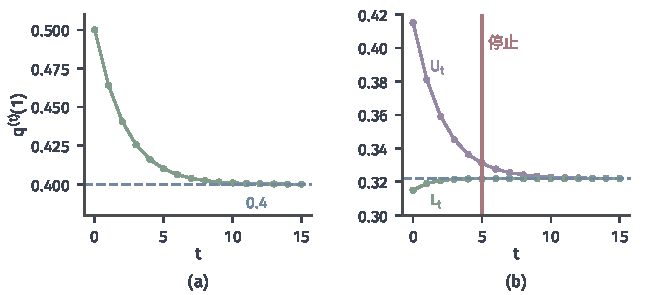
\includegraphics[width=110mm]{figures/07-probability/06-channel-coding/matplotlib/dcc-ba-z/figure.pdf}
 \caption{Z信道上从$q_0=(\tfrac12,\tfrac12)$出发的Blahut–Arimoto迭代。(a) 绿点为$q_t(1)$，蓝色虚线为最优值$0.4$；(b) 紫线为上界$U_t$，绿线为下界$L_t$，蓝色虚线为容量$\log_2(5/4)$，红线标出第一次满足$U_t-L_t\leq0.01$的轮次$t=5$。}
 \label{fig:dcc-ba-z}
\end{BookInlineFigure}

\paragraph{收敛性}
下界的收敛可以完整证明，并且给出速度。

\begin{theorem}[Blahut–Arimoto迭代的收敛]
\label{thm:dcc-ba-convergence}
设$q_0$的支撑是整个$\mathcal{X}$，$q^{*}$是任一最优输入分布。则$I(q_t)$与$L_t$都单调不减，并且
\begin{equation}
 C-L_T\leq\frac{D_{\mathrm{KL}}(q^{*}\Vert q_0)}{T+1},\qquad T=0,1,2,\dots .
 \label{eq:dcc-ba-rate}
\end{equation}
$q_0$均匀时右边不超过$\log_2\lvert\mathcal{X}\rvert/(T+1)$。
\end{theorem}

\begin{proof}
单调性。记$r_t=r_{q_t}$。由$J$对两个变量分别取最大的性质，
\[
 \begin{aligned}
 I(q_t)=J(q_t,r_t)&\leq J(q_{t+1},r_t)=L_t\\
 &\leq J(q_{t+1},r_{t+1})=I(q_{t+1})\leq J(q_{t+2},r_{t+1})=L_{t+1} .
 \end{aligned}
\]

速度。更新公式~\eqref{eq:dcc-ba-update}的对数形式是$\log_2\frac{q_{t+1}(x)}{q_t(x)}=D_t(x)-L_t$；$q_0$处处为正，每步乘以正数，所以$q_t$处处为正。按$q^{*}$求平均，
\[
 \sum_xq^{*}(x)\log_2\frac{q_{t+1}(x)}{q_t(x)}=\sum_xq^{*}(x)D_t(x)-L_t .
\]
定理~\ref{thm:dcc-kkt}证明中的恒等式（取$q=q^{*}$、$r=p_t$）给出
\[
 \sum_xq^{*}(x)D_t(x)=C+D_{\mathrm{KL}}(p^{*}\Vert p_t)\geq C ,
\]
所以右边不小于$C-L_t$。对$t=0,\dots,T$求和，左边逐项相消，
\[
 \begin{aligned}
 D_{\mathrm{KL}}(q^{*}\Vert q_0)-D_{\mathrm{KL}}(q^{*}\Vert q_{T+1})&=\sum_{t=0}^{T}\sum_xq^{*}(x)\log_2\frac{q_{t+1}(x)}{q_t(x)}\\
 &\geq\sum_{t=0}^{T}(C-L_t)\geq(T+1)(C-L_T) ,
 \end{aligned}
\]
最后一步用了$L_t$单调不减。$D_{\mathrm{KL}}(q^{*}\Vert q_{T+1})\geq0$，移项即得式~\eqref{eq:dcc-ba-rate}。均匀初始时
\[
 D_{\mathrm{KL}}(q^{*}\Vert q_0)=\log_2\lvert\mathcal{X}\rvert-H(q^{*})\leq\log_2\lvert\mathcal{X}\rvert .
\]
\end{proof}

上界$U_t$同样收敛到$C$，因为$p_t$收敛到唯一的最优输出分布；这一部分的证明更长，可查阅~\scite{math-cover2006information}。实践中不需要它的速度：只要算出$U_t$与$L_t$，区间$[L_t,U_t]$本身就是可验证的结论。

\paragraph{初始支撑与零概率输入}
证明中“$q_0$处处为正”不可省略。若$q_0(x)=0$，乘性更新使$q_t(x)$永远为零，迭代实际是在去掉输入$x$的信道上进行；若$x$是有用的输入，迭代会收敛到一个偏小的值。这时上界会暴露问题：$U_t$对全部输入取最大值，包括概率为零的输入，于是差距$U_t-L_t$不会趋于零。同样的原因，初始支撑完整时$p_t(y)>0$对一切可能出现的输出成立，散度不会出现除以零。

反过来，最优输入可能给某些符号零概率，迭代却只能让它们的概率趋于零而不能到达零。考虑三输入二输出的信道，三行为$(1,0)$、$(0,1)$、$(\tfrac12,\tfrac12)$：前两个输入无噪声，第三个输入的输出与输入无关。容量为$1$比特，最优输入是$(\tfrac12,\tfrac12,0)$。从均匀分布出发，由对称性$p_t=(\tfrac12,\tfrac12)$始终不变，散度始终为$(1,1,0)$，每轮第三个分量相对其余两个缩小一半：
\[
 q_t(2)=\frac{1}{2^{t+1}+1}:\qquad \tfrac13,\ \tfrac15,\ \tfrac19,\ \tfrac1{17},\ \dots
\]
上界从第$0$轮起就等于$1$，下界$L_t=\log_2(2-q_t(2))$的差距按几何速度缩小，远快于式~\eqref{eq:dcc-ba-rate}保证的$\log_23/(t+1)$。图~\ref{fig:dcc-ba-support}画出这两点。

\begin{BookInlineFigure}
 \centering
 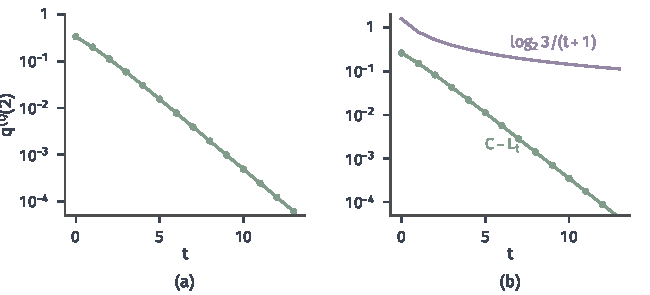
\includegraphics[width=110mm]{figures/07-probability/06-channel-coding/matplotlib/dcc-ba-support/figure.pdf}
 \caption{三行分别为$(1,0)$、$(0,1)$、$(\tfrac12,\tfrac12)$的信道上，从均匀分布出发的Blahut–Arimoto迭代，纵轴均为对数坐标。(a) 无用输入的概率$q_t(2)=1/(2^{t+1}+1)$按几何速度减小，但始终为正；(b) 绿线为下界的差距$C-L_t$，紫线为定理~\ref{thm:dcc-ba-convergence}的保证$\log_23/(t+1)$；上界$U_t$从第$0$轮起就等于$C=1$。}
 \label{fig:dcc-ba-support}
\end{BookInlineFigure}

这个例子说明两件事。第一，概率很小不等于应当为零，不能仅凭$q_t(x)$小就把输入删掉；需要删减时，应先用上下界确认删去后容量不变。第二，迭代变化小也不是停止的依据。Z信道第$7$轮以后$q_t$每轮只变化约$0.002$，差距仍有$0.004$；在收敛更慢的信道上，变化可以极小而离最优仍远。应当用的是$U_t-L_t$。

\paragraph{计算量}
每轮需要算$p_t=q_t\bm{W}$与全部散度，各需要$O(\lvert\mathcal{X}\rvert\lvert\mathcal{Y}\rvert)$次运算，更新与求界只需$O(\lvert\mathcal{X}\rvert)$。由式~\eqref{eq:dcc-ba-rate}，下界达到精度$\tau$至多需要约$\log_2\lvert\mathcal{X}\rvert/\tau$轮；实际中常快得多。

\paragraph{带成本约束的迭代}
对第~\ref{sec:dcc-costs}节的问题，先固定乘子$s\geq0$，求式~\eqref{eq:dcc-lagrangian}中的最大化。推导与上面相同，只是$a(x)$多了一项$-s\,c(x)$，更新变为
\begin{equation}
 q_{t+1}(x)\propto q_t(x)\,2^{D_t(x)-s\,c(x)} .
 \label{eq:dcc-ba-cost-update}
\end{equation}
固定$s$迭代到收敛，得到$C(\Gamma)$曲线上斜率为$s$的点：其横坐标是平均成本$\Gamma(s)=\sum_xq(x)c(x)$，纵坐标是$I(q)$。$s$越大，成本越受惩罚，$\Gamma(s)$越小。要对给定的$\Gamma$求$C(\Gamma)$，就在外层对$s$二分，使$\Gamma(s)$等于$\Gamma$。

图~\ref{fig:dcc-ba-cost}在Z信道上取$s=0,0.1,\dots,1.5$，各迭代$400$轮，得到的点都落在解析曲线$h_2(\Gamma/2)-\Gamma$上；对$\Gamma=0.25$二分得到$s\approx0.4037$，与第~\ref{sec:dcc-cost-capacity}小节算出的切线斜率一致。$s=0$给出无约束的最优点$\Gamma=0.4$。

\begin{BookInlineFigure}
 \centering
 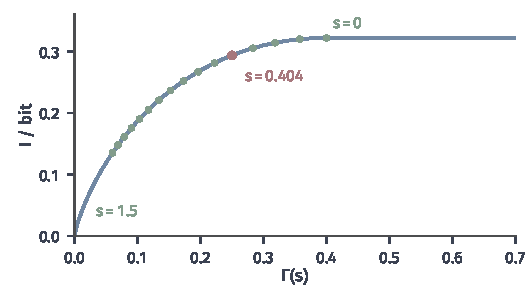
\includegraphics[width=90mm]{figures/07-probability/06-channel-coding/matplotlib/dcc-ba-cost/figure.pdf}
 \caption{Z信道、成本$c(0)=0$、$c(1)=1$时带乘子的Blahut–Arimoto迭代。蓝线为容量—成本函数的解析式，绿点为$s=0,0.1,\dots,1.5$各自迭代$400$轮得到的$(\Gamma(s),I)$，红点为二分求得的$s\approx0.404$，对应预算$\Gamma=0.25$。}
 \label{fig:dcc-ba-cost}
\end{BookInlineFigure}

带约束时，误差保证也要相应修改。上界来自弱对偶~\eqref{eq:dcc-weak-duality}：用定理~\ref{thm:dcc-kkt}中的恒等式，对任意$q$有
\[
 I(q)-s\sum_xq(x)c(x)\leq\max_x\bigl[D_{\mathrm{KL}}(W_x\Vert p_t)-s\,c(x)\bigr] ,
\]
所以
\[
 C(\Gamma)\leq\max_x\bigl[D_t(x)-s\,c(x)\bigr]+s\Gamma ,
\]
对任意$s\geq0$与任意一轮都成立。下界是当前输入的互信息$I(q_t)$，但只有在$\sum_xq_t(x)c(x)\leq\Gamma$时才算数：二分得到的$s$只使预算近似满足，若$q_t$略微超支，它的互信息不是$C(\Gamma)$的下界。所以报告结果时要同时核对实际的平均成本，必要时把$s$稍微调大，换取一个严格可行的输入。
